% ── Chapter 3: Methodology ───────────────────────────────────

\chapter{Methodology}

This chapter describes how the framework was actually built, from
hardware selection to software deployment. The work proceeded in four
phases: (i) assembling the mobile chassis and validating all hardware
through a web-based manual teleoperation interface, (ii) collecting a
path image dataset, training and optimising a YOLOv8 segmentation model,
and deploying it on the Pi~5, (iii) implementing the autonomous
PID-based navigation stack with trajectory logging, and (iv) building
the environmental monitoring pipeline with multi-channel cloud
communication. Each phase built on the previous one, so by the time
autonomous operation was tested, the hardware and communication
infrastructure were already known to be working correctly.

Figure~\ref{fig:sysarch} presents the overall system architecture of
the proposed framework. The diagram is divided into two major
subsystems: the Environment Monitoring System at the top and the
Autonomous Robot System at the bottom. The environment monitoring
subsystem consists of a DHT11 temperature and humidity sensor and an
MQ135 air quality sensor, both connected to an Arduino UNO
microcontroller. The Arduino transmits sensor readings over a USB
serial connection to a Raspberry Pi~3. The Raspberry Pi~3 processes
the sensor data and manages all cloud communication. The autonomous
robot subsystem is built around a Raspberry Pi~5 connected to a camera,
an HC-SR04 ultrasonic sensor, an active buzzer, a PCA9685 PWM driver,
and four continuous-rotation servo motors. The environment monitoring
subsystem is physically mounted on the autonomous robot chassis,
forming a single integrated mobile platform. This separation of
processing responsibilities between the Raspberry Pi~3 and the
Raspberry Pi~5 ensures that each subsystem operates independently
without interfering with the other.

\begin{figure}[tbp]
  \centering
  \makebox[\textwidth][c]{%
    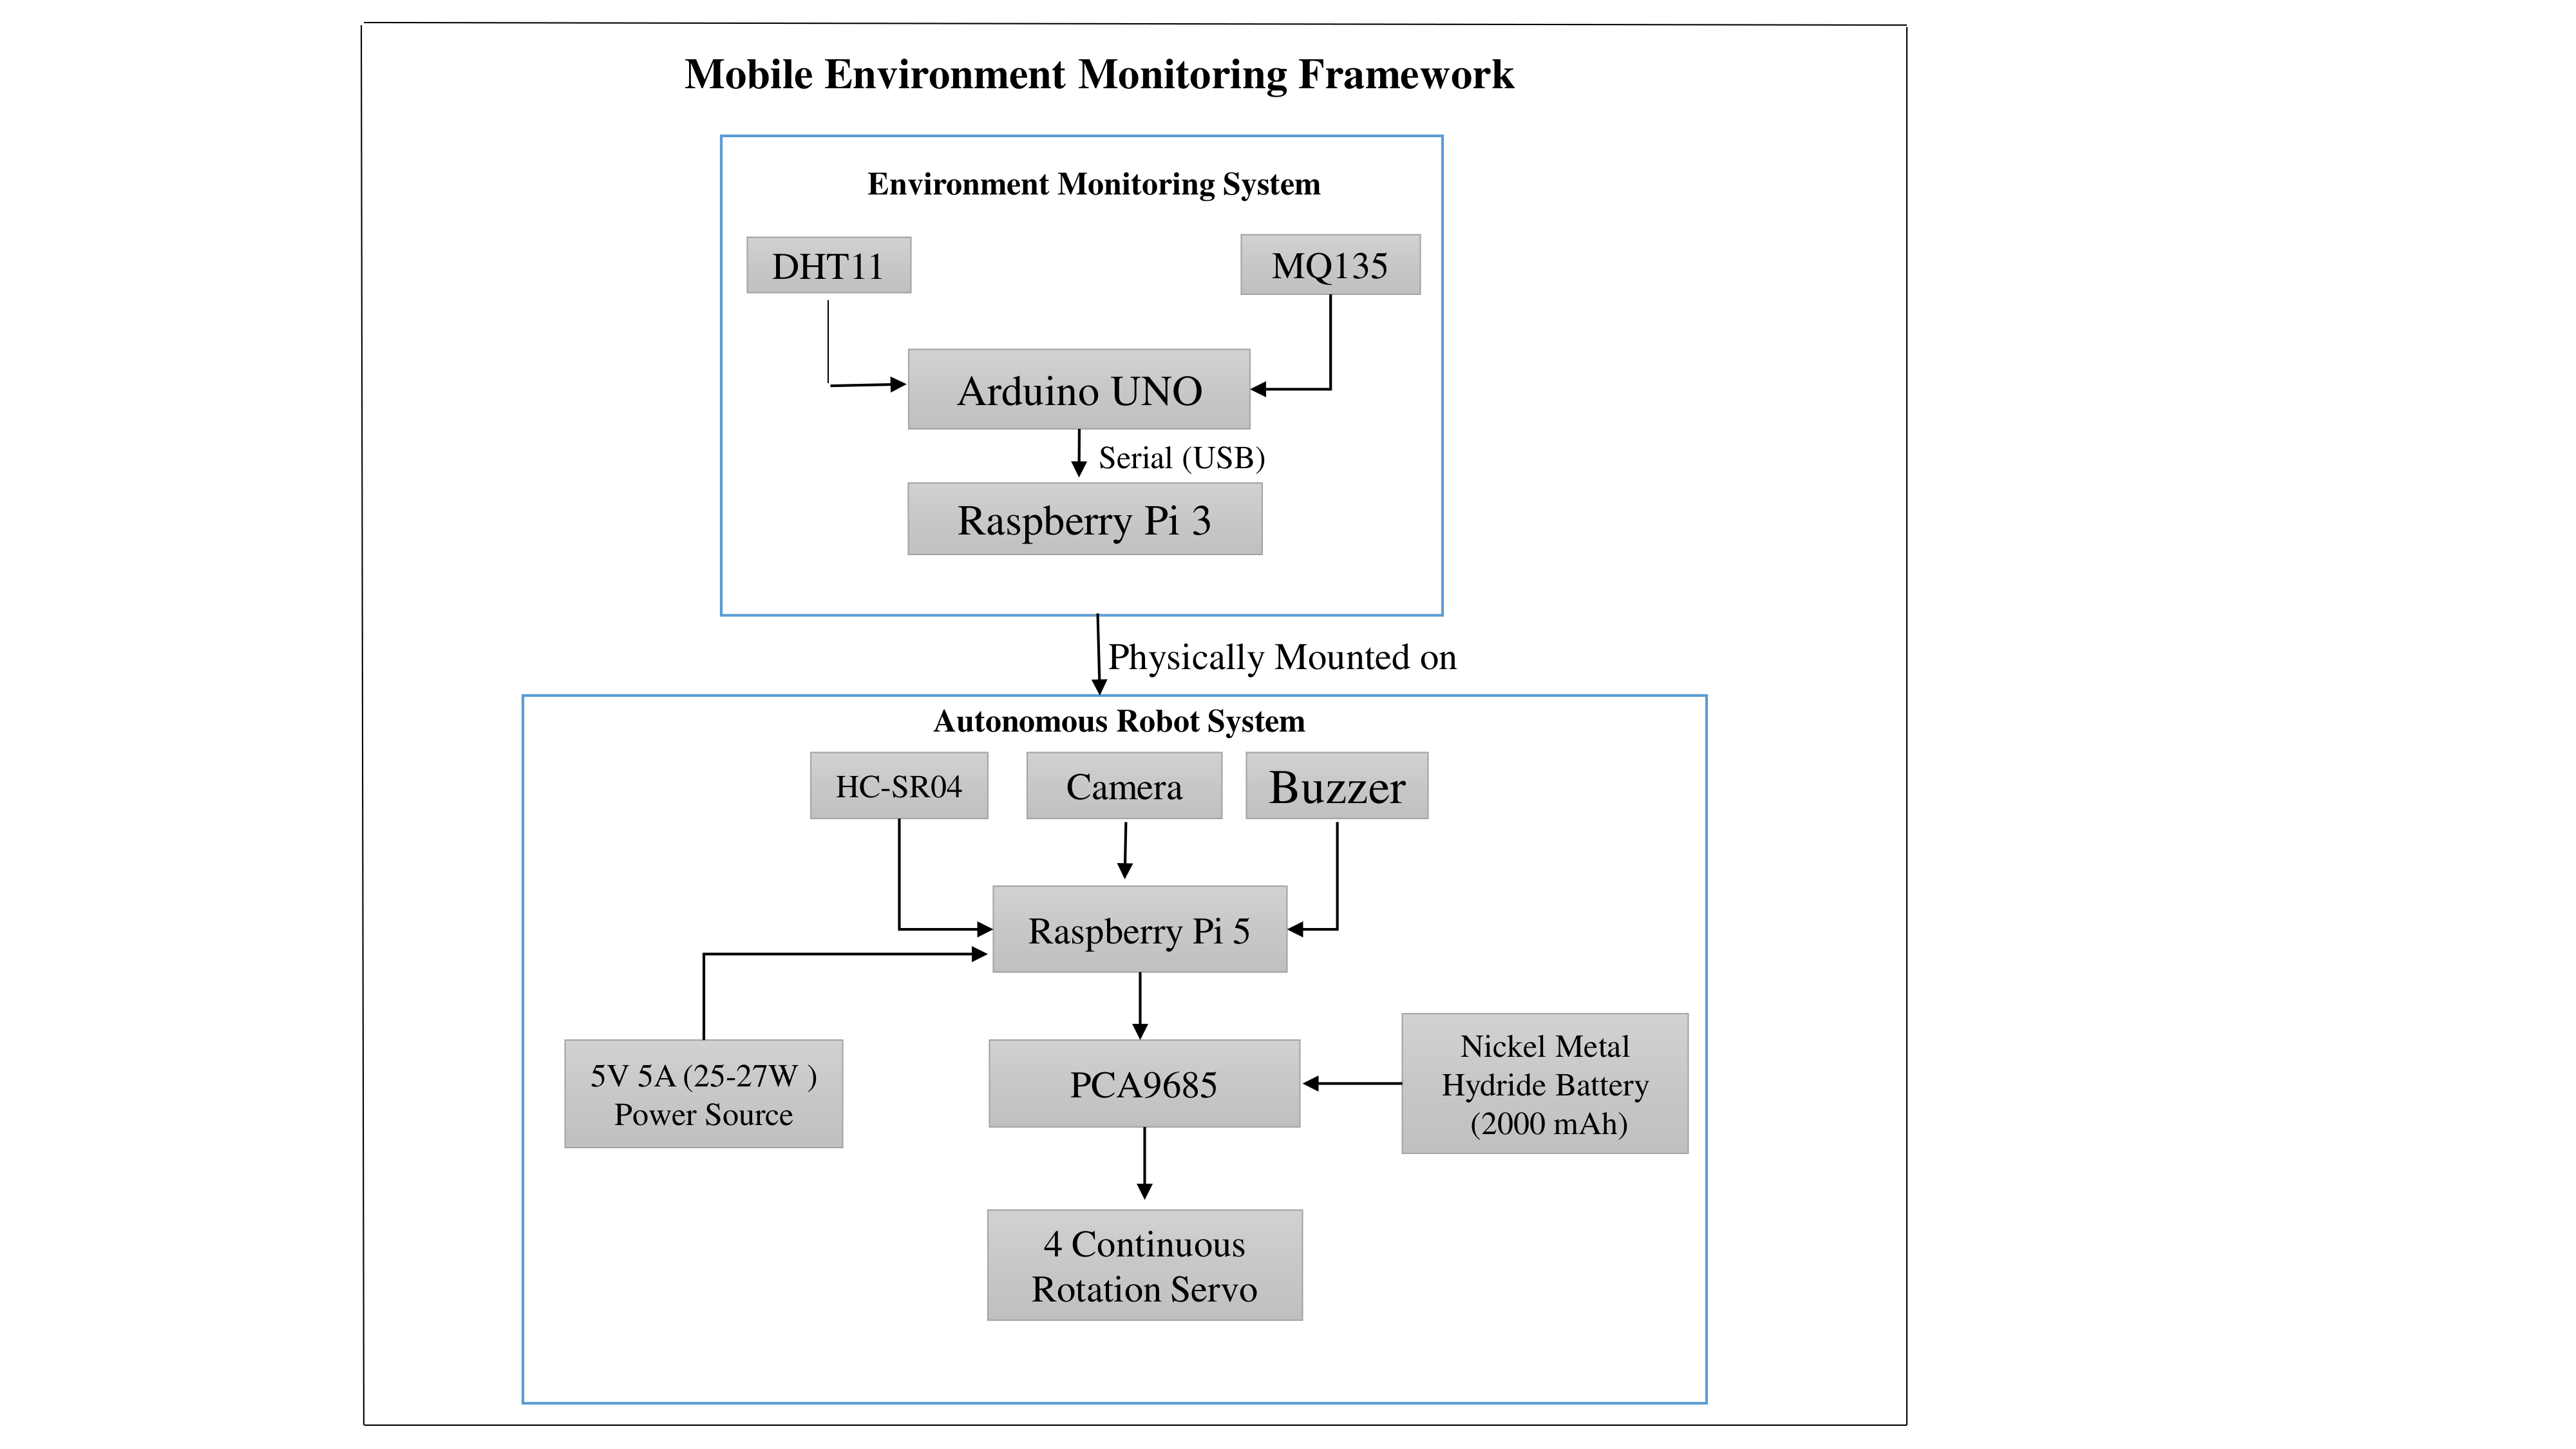
\includegraphics[width=1.4\textwidth]{system_architecture.png}%
  }
  \caption{Overall system architecture of the proposed framework.}
  \label{fig:sysarch}
\end{figure}

\section{Hardware Design and Manual Robot Construction}

The mobile platform constitutes the physical foundation of the
framework. A four-wheel differential-drive chassis was selected for
its mechanical simplicity, ease of control, and established suitability
for structured indoor navigation tasks \cite{r10,r11}. This choice
is consistent with the majority of experimental mobile robot platforms
reported in the literature \cite{r9,r18}.

\subsection{Mechanical Platform and Drive System}

Four continuous-rotation servo motors serve as drive actuators, mounted
on a rigid aluminium chassis with two motors per side. The servo motors
are controlled through a PCA9685 16-channel PWM driver
operating at 50\,Hz over the I$^2$C bus of the Raspberry Pi~5 \cite{r38}.
The PCA9685 generates pulse-width modulated signals in the range
1000--2000\,$\mu$s, where a centre pulse of 1600\,$\mu$s corresponds
to the stationary state, values above 1600\,$\mu$s command forward
rotation, and values below 1600\,$\mu$s command reverse rotation.
Individual calibration factors are applied to each motor channel to
compensate for mechanical asymmetries arising from servo manufacturing
tolerances.

Table~\ref{tab:motor} lists the four motor channels with their
respective chassis positions, rotation directions, and calibration
factors. Channel 0 drives the rear right motor in the normal direction
with a calibration factor of 1.335, while channel 1 drives the rear
left motor in the reversed direction with a factor of 0.790. Channel 2
drives the front right motor in the normal direction and requires the
highest calibration factor of 2.335, and channel 3 drives the front
left motor in the reversed direction with a factor of 0.290. These
asymmetric factors reflect the physical differences between the four
servo units and were determined empirically to achieve straight-line
motion on a flat surface.

\begin{table}[tbp]
  \centering
  \caption{Motor channel assignments and calibration factors.}
  \label{tab:motor}
  \begin{tabular}{cccc}
    \toprule
    Channel & Position    & Direction & Calibration Factor \\
    \midrule
    0       & Rear Right  & Normal    & 1.335 \\
    1       & Rear Left   & Reversed  & 0.790 \\
    2       & Front Right & Normal    & 2.335 \\
    3       & Front Left  & Reversed  & 0.290 \\
    \bottomrule
  \end{tabular}
\end{table}

\subsection{Sensing and Perception Hardware}

The following sensors and peripheral devices are integrated onto the
robot platform.

The HC-SR04 ultrasonic sensor is mounted at the front lower
section of the chassis, connected to GPIO pin 23 (TRIG) and GPIO pin
24 (ECHO) of the Raspberry Pi~5 \cite{r34}. The sensor emits 40\,kHz
ultrasonic pulses and computes obstacle distance from the echo return
time. Any measurement below 20\,cm triggers automatic forward-motion
blocking and activates the buzzer alert.

The Logitech Brio 100 USB Camera is mounted centrally on a
forward-facing bracket above the chassis at a height of 20\,cm above
the floor surface, angled 45$^\circ$ downward toward the path. The
camera captures frames at a resolution of 640$\times$480 pixels at 30
frames per second through the device node \texttt{/dev/video0}. This
mounting configuration ensures that the path tape is fully within the
camera field of view at the operating height.

The active buzzer is connected to GPIO pin 18 and is activated
by the obstacle detection thread whenever an object is detected within
the 20\,cm safety threshold.

The power supply consists of a dedicated 5\,V, 5\,A
(25--27\,W) regulated unit powering the Raspberry Pi~5 and the PCA9685
driver, and a separate 2000\,mAh Nickel Metal Hydride battery pack
powering the four servo motors. This separation isolates motor current
transients from the logic supply rail, preventing voltage fluctuations
from disrupting the Raspberry Pi~5 during rapid motor direction changes.

Figure~\ref{fig:robot} shows the fully assembled robot platform. The
Logitech Brio 100 camera is visible at the top centre of the chassis
body. The HC-SR04 ultrasonic sensor is mounted at the front lower
section facing forward.

\begin{figure}[tbp]
  \centering
  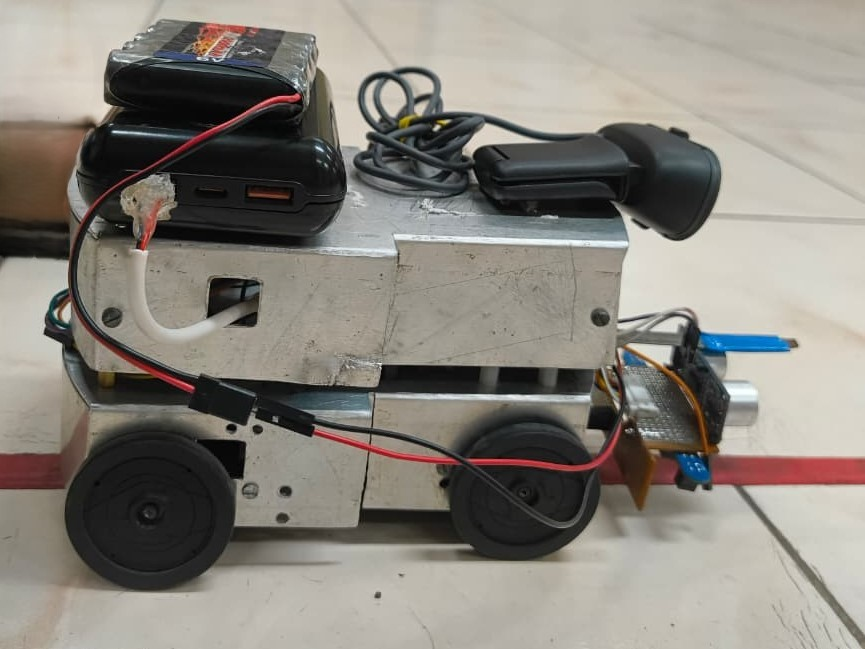
\includegraphics[width=0.85\textwidth]{WhatsApp Image 2026-04-10 at 1.09.05 PM (2).jpeg}
  \caption{Assembled mobile robot platform showing the Logitech Brio~100
  camera mounted at the top centre, the HC-SR04 ultrasonic sensor at
  the front lower section.}
  \label{fig:robot}
\end{figure}

\subsection{Web-Based Manual Control System}

Prior to the deployment of autonomous navigation software, a
web-based teleoperation interface was implemented to verify motor
functionality, sensor integration, and hardware communication under
manual human supervision \cite{r2}. The backend is implemented as a
Flask RESTful application \cite{r37} exposing dedicated API endpoints
for directional commands (forward, backward, left, right, and stop)
and variable speed control. A responsive HTML, CSS, and JavaScript
dashboard is served at \texttt{http://<Pi-IP>:5000} and is accessible
from any device connected to the same local network. The interface
supports button-based, touch-based, and keyboard-based controls using
the W/A/S/D key set and directional arrow keys. A multi-threaded
software architecture ensures that the motor command thread, obstacle
monitoring thread, and Flask HTTP serving thread execute concurrently
without blocking one another. This phase validated mechanical
operability and sensor responsiveness before the autonomous control
stack was deployed.

\section{Path Dataset Collection and YOLOv8 Model Training}

\subsection{Path Design and Data Collection}

A navigable path was constructed using red adhesive tape laid
on tiled and concrete floor surfaces within the laboratory environment
at the Central Scientific and Industrial Research -- Central Mechanical
Engineering Research Institute. Red tape was selected because it provides
high colour contrast against typical indoor floor colours under both
natural daylight and artificial fluorescent lighting conditions. The
Logitech Brio 100 camera was mounted at 20\,cm above the floor surface
and angled 45$^\circ$ downward, capturing images at a resolution of
640$\times$480 pixels. A total of 289 images were collected, covering
three path geometry categories: straight sections at 40\%, curved
sections at 35\%, and complex turns with direction changes at 25\%.
Lighting conditions were varied to include well-lit (60\%), low-light
(25\%), and mixed shadow (15\%) scenarios, ensuring dataset diversity
for robust model generalisation \cite{r32,r31}.

\subsection{Image Annotation and Dataset Preparation}

Each of the 289 captured images was annotated using the
Computer Vision Annotation Tool (CVAT) platform \cite{r31}.
Polygon annotations were drawn manually around the navigable path
region in each image frame, labelling the path foreground as class
\texttt{path} (class index 0). The annotations were exported in YOLO
segmentation format and validated through visual inspection. Ambiguous
or low-quality samples were removed during the inspection pass. The
dataset was then partitioned into three splits using a 70/20/10 ratio.

Table~\ref{tab:split} presents the resulting split distribution. The
training split contains 202 images and 202 corresponding label files.
The validation split contains 57 images and labels, and the test split
contains 30 images and labels.

\begin{table}[tbp]
  \centering
  \caption{Dataset split distribution.}
  \label{tab:split}
  \begin{tabular}{ccc}
    \toprule
    Split      & Images & Labels \\
    \midrule
    Training   & 202    & 202 \\
    Validation & 57     & 57 \\
    Test       & 30     & 30 \\
    \midrule
    Total      & 289    & 289 \\
    \bottomrule
  \end{tabular}
\end{table}

\subsection{Model Architecture}

The YOLOv8n-seg (nano segmentation) variant of the YOLOv8
architecture was selected as the segmentation model \cite{r32}.
The model contains 86 fused layers with 3,258,259 parameters,
zero gradients in inference mode, and a computational cost of
11.3~GFLOPs.

The YOLOv8 family provides five model scale variants ---
nano~(n), small~(s), medium~(m), large~(l), and extra-large~(x)
--- each progressively increasing in parameter count, computational
cost, and reported accuracy on standard benchmarks \cite{r32}.
Table~\ref{tab:yolov8compare} presents a comparison of the five
variants on the COCO dataset alongside their approximate CPU inference
performance on an embedded single-board computer.

\begin{table}[tbp]
  \centering
  \caption{YOLOv8 segmentation variant comparison (COCO val2017) \cite{r32}.}
  \label{tab:yolov8compare}
  \begin{tabular}{lcccc}
    \toprule
    Variant        & Params (M) & GFLOPs & Mask mAP@50-95 & CPU Latency \\
    \midrule
    YOLOv8n-seg    & 3.4        & 12.6   & 36.7           & $\sim$65\,ms \\
    YOLOv8s-seg    & 11.8       & 42.6   & 42.6           & $\sim$190\,ms \\
    YOLOv8m-seg    & 27.3       & 110.2  & 49.9           & $\sim$440\,ms \\
    YOLOv8l-seg    & 46.0       & 220.5  & 52.3           & $\sim$870\,ms \\
    YOLOv8x-seg    & 71.8       & 344.1  & 53.4           & $>$1200\,ms  \\
    \bottomrule
    \multicolumn{5}{l}{\small CPU latency measured on a Raspberry Pi~5 at 320$\times$320 resolution.}
  \end{tabular}
\end{table}

As Table~\ref{tab:yolov8compare} shows, the larger variants (YOLOv8s
through YOLOv8x) achieve higher mask mAP@50-95 values on the
general COCO benchmark, ranging from 42.6 to 53.4. However, their
CPU latencies on the Raspberry Pi~5 at 320$\times$320 resolution
range from approximately 190\,ms to over 1200\,ms, corresponding to
frame rates of 5.3\,FPS down to below 1\,FPS. None of these variants
can sustain the minimum 15\,FPS required for stable closed-loop PID
control on the Raspberry Pi~5 CPU \cite{r34,r29}. The nano variant,
by contrast, achieves 15.4\,FPS after ONNX conversion, as demonstrated
in the benchmarking results in Section~\ref{sec:opt}, and this is the
only variant that clears the real-time threshold on the available
embedded hardware.

The task addressed in this work is fundamentally simpler than the
general COCO benchmark: the model is required to segment a single
highly distinctive class (red adhesive tape) under controlled
indoor lighting against a uniform tiled background. In this specific
setting, a high generalisation capacity is not required and the
performance gap between nano and larger variants is expected to
narrow substantially with fine-tuning \cite{r30,r32}. The trained
YOLOv8n-seg model achieved a mask mAP@50 of 0.988 on the
57-image validation split, which exceeds the mAP@50 values reported
for the larger variants on COCO, confirming that for this task
the nano variant provides accuracy that is more than sufficient.

The nano variant was therefore selected on the following grounds:

\begin{itemize}
  \item Only the nano variant meets the real-time constraint of
        15\,FPS on the Raspberry Pi~5 CPU after ONNX conversion.
  \item The task involves segmenting a single, visually distinctive
        class, which does not require the generalisation capacity
        of larger models.
  \item The fine-tuned model achieves 0.988 mask mAP@50, which is
        sufficient for reliable closed-loop path following.
  \item The lower parameter count (3.4~M) reduces memory footprint
        to 280\,MB at 320$\times$320, within the operational limit
        of the 4\,GB Raspberry Pi~5 \cite{r34}.
\end{itemize}

The model accepts a single class label (\texttt{path}) and produces
instance segmentation masks together with bounding boxes at each
inference step \cite{r12,r13,r29}.

\subsection{Training Configuration and Procedure}

Training was performed on Google Colab using a Tesla T4 GPU (15095\,MB
VRAM) with the Ultralytics 8.4.7 framework \cite{r32} under PyTorch
2.9.0 with CUDA 12.6.

Table~\ref{tab:training} presents the complete training configuration.
Training ran for a maximum of 200 epochs with an early stopping patience
of 30 epochs, meaning training was terminated if the validation mAP did
not improve for 30 consecutive epochs. A batch size of 8 was used with
the Adam optimizer and an initial and final learning rate of 0.01. The
model was initialised from the official pretrained \texttt{yolov8n-seg.pt}
weights and fine-tuned on the custom path dataset. Mixed-precision
automatic mixed precision (AMP) training was enabled. Data augmentation
included mosaic augmentation at probability 1.0, horizontal flip at
0.5, HSV hue, saturation and value shifts, translation of 0.1, and
scale variation of 0.5. The warmup phase ran for 3 epochs.

\begin{table}[tbp]
  \centering
  \caption{YOLOv8n-seg training configuration.}
  \label{tab:training}
  \begin{tabular}{ll}
    \toprule
    Parameter               & Value \\
    \midrule
    Epochs                  & 200 \\
    Early stopping patience & 30 epochs \\
    Batch size              & 8 \\
    Input resolution        & 640$\times$640 \\
    Optimizer               & Adam \\
    Initial learning rate   & 0.01 \\
    Final learning rate     & 0.01 \\
    Momentum                & 0.937 \\
    Weight decay            & 0.0005 \\
    Warmup epochs           & 3 \\
    Mosaic augmentation     & 1.0 \\
    Horizontal flip         & 0.5 \\
    HSV-Hue                 & 0.015 \\
    HSV-Saturation          & 0.7 \\
    HSV-Value               & 0.4 \\
    Translation             & 0.1 \\
    Scale                   & 0.5 \\
    Pretrained weights      & yolov8n-seg.pt \\
    Mixed precision (AMP)   & Enabled \\
    \bottomrule
  \end{tabular}
\end{table}

\subsection{Validation Results}

The trained model was evaluated on the 57-image validation split
immediately after training. Table~\ref{tab:val} presents the validation
metrics across both the bounding box detection task and the instance
segmentation mask task. For the bounding box task, the model achieved a
precision of 0.947, a recall of 0.946, an mAP@50 of 0.973, and an
mAP@50-95 of 0.821. For the segmentation mask task, precision was 0.965,
recall was 0.963, mAP@50 was 0.988, and mAP@50-95 was 0.736. The mask
mAP@50 of 0.988 indicates that the model reliably segments the red tape
path in 96 out of every 100 validation frames at the standard IoU
threshold. The best checkpoint was saved to \texttt{best.pt} based on
the highest validation mAP@50.

\begin{table}[tbp]
  \centering
  \caption{YOLOv8n-seg validation metrics on the 57-image validation split.}
  \label{tab:val}
  \begin{tabular}{lcccc}
    \toprule
    Task  & Precision & Recall & mAP@50 & mAP@50-95 \\
    \midrule
    Box   & 0.947     & 0.946  & 0.973  & 0.821 \\
    Mask  & 0.965     & 0.963  & 0.988  & 0.736 \\
    \bottomrule
  \end{tabular}
\end{table}

\subsection{Model Optimisation for Embedded Deployment}
\label{sec:opt}

Direct deployment of the trained PyTorch \texttt{best.pt} model on the
Raspberry Pi~5 CPU at 640$\times$640 resolution produced an average
inference time of 101.6\,ms, corresponding to 9.8 frames per second.
This throughput is insufficient for stable closed-loop control, which
requires a sustained minimum of 10 to 15 frames per second
\cite{r29,r10}. A two-stage optimisation pipeline was applied to meet
this requirement.

\paragraph{Stage 1: Resolution Tuning.}
Inference resolution was benchmarked at three settings on the
Raspberry Pi~5 (Broadcom BCM2712, quad-core Cortex-A76 at 2.4\,GHz,
4\,GB LPDDR4X RAM, ONNX Runtime 1.23.2) using 20 inference iterations
per configuration. As shown in Table~\ref{tab:bench}, at 640$\times$640
resolution, inference takes 101.6\,ms on average, yielding 9.8\,FPS
with a memory footprint of 450\,MB. Reducing resolution to
480$\times$480 increases the average inference time to 201.3\,ms,
reducing throughput to 5.0\,FPS. At 320$\times$320, inference time
is 103.0\,ms, yielding 9.7\,FPS with a reduced memory footprint of
280\,MB.

\begin{table}[tbp]
  \centering
  \caption{Resolution benchmarking on Raspberry Pi~5 in PyTorch format.}
  \label{tab:bench}
  \begin{tabular}{cccc}
    \toprule
    Resolution       & Average Inference Time & FPS & Memory Usage \\
    \midrule
    640$\times$640   & 101.6\,ms              & 9.8 & 450\,MB \\
    480$\times$480   & 201.3\,ms              & 5.0 & 350\,MB \\
    320$\times$320   & 103.0\,ms              & 9.7 & 280\,MB \\
    \bottomrule
  \end{tabular}
\end{table}

\paragraph{Stage 2: ONNX Conversion.}
The best checkpoint was exported from PyTorch to ONNX format at a
fixed static input shape of 320$\times$320 using the Ultralytics ONNX
export pipeline \cite{r33}. Inference was executed using ONNX Runtime
with \texttt{CPUExecutionProvider}. As shown in Table~\ref{tab:onnx},
the ONNX model reduces average inference time from 103.0\,ms to
64.8\,ms, increasing throughput from 9.7\,FPS to 15.4\,FPS,
representing a speedup factor of 1.57$\times$ over the PyTorch baseline.

\begin{table}[tbp]
  \centering
  \caption{PyTorch versus ONNX inference comparison at 320$\times$320.}
  \label{tab:onnx}
  \begin{tabular}{ccccc}
    \toprule
    Format  & Resolution     & Average Time & FPS  & Speedup \\
    \midrule
    PyTorch & 320$\times$320 & 103.0\,ms    & 9.7  & 1.0$\times$ \\
    ONNX    & 320$\times$320 & 64.8\,ms     & 15.4 & 1.57$\times$ \\
    \bottomrule
  \end{tabular}
\end{table}

The FPS progression across all four model configurations is illustrated
in Figure~\ref{fig:tradeoff}, which plots FPS on the vertical axis
against four model configurations: 640 PyTorch, 480 PyTorch, 320
PyTorch, and 320 ONNX. The figure confirms that ONNX conversion at
320$\times$320 resolution is the only configuration that meets the
real-time threshold of 15 FPS, making format conversion the decisive
optimisation step.

\begin{figure}[tbp]
  \centering
  \includegraphics[width=0.88\textwidth]{accuracy_speed_tradeoff.png}
  \caption{FPS comparison across all four model configurations
  (640 PyTorch, 480 PyTorch, 320 PyTorch, 320 ONNX) on the
  Raspberry Pi~5 CPU, confirming that ONNX at 320$\times$320 is the
  only configuration meeting the 15\,FPS real-time threshold.}
  \label{fig:tradeoff}
\end{figure}

A 30-minute continuous stability test confirmed an average throughput
of $15.2 \pm 0.8$ FPS, a peak of 16.8 FPS, a minimum of 13.9 FPS,
zero memory leaks, and a CPU temperature stable at $68 \pm 2\,^\circ$C
without thermal throttling. The optimised model was saved as
\texttt{best\_320.onnx} and deployed to the \texttt{models/} directory
on the Raspberry Pi~5.

\section{Autonomous Path-Following System}

\subsection{Control Flow Overview}

The control flow of the complete autonomous path-following system is
illustrated in Figure~\ref{fig:robotflow}. The flowchart describes the
sequential and conditional logic that governs robot behaviour from
startup to shutdown.

The following steps describe the sequential and conditional logic
executed by the robot during each autonomous cycle:

\begin{enumerate}

  \item \emph{Start.} The system begins execution when the operator
        issues a START command through the web dashboard.

  \item \emph{Initialise camera, motors, and sensors.} The Raspberry
        Pi~5 opens the camera stream at 640$\times$480 resolution,
        initialises the I$^2$C connection to the PCA9685, and confirms
        GPIO pin assignments for the HC-SR04 and buzzer.

  \item \emph{Capture frame from camera.} At each iteration of the
        vision loop running at 20\,Hz, a single frame is captured from
        the camera buffer.

  \item \emph{Run YOLO segmentation.} The captured frame is resized
        to 320$\times$320 pixels and passed to the ONNX Runtime session.
        The model produces an instance segmentation mask for the
        \texttt{path} class and a confidence score.

  \item \emph{Is path detected?} The YOLO output is checked for valid
        detections within the region of interest (bottom 30\% of frame).
        If no detection is present, the robot is stopped and the vision
        loop returns to step~3 to attempt path reacquisition.

  \item \emph{Calculate centroid.} If a valid path detection is present,
        the centroid of the segmentation mask within the ROI is computed,
        representing the horizontal centre of the detected path.

  \item \emph{Compute error (deviation).} The horizontal centroid
        position is compared to the horizontal centre of the camera
        frame. The difference is normalised to the range
        $[-1.0,\,+1.0]$ and constitutes the path deviation error
        signal $e(t)$.

  \item \emph{Apply deadband.} A deadband filter of $\pm 0.04$ is
        applied to the deviation signal to prevent the PID controller
        from generating unnecessary steering corrections on
        near-straight sections.

  \item \emph{Read ultrasonic sensor.} The HC-SR04 sensor is triggered
        and the echo pulse duration is converted to distance in
        centimetres.

  \item \emph{Is obstacle detected?} The measured distance is compared
        to the 20\,cm safety threshold. If an obstacle is present,
        all motor channels are set to neutral and the buzzer is
        activated.

  \item \emph{Apply PID control.} If no obstacle is detected, the
        deadband-filtered error $e(t)$ is processed by the PID
        controller using Equation~\eqref{eq:pid} with gains
        $K_p = 13.2$, $K_i = 0.0$, and $K_d = 0.475$.

  \item \emph{Send signal to motor driver.} The steering correction
        $u(t)$ from Equation~\eqref{eq:pid} is combined with the base
        forward speed. Per-wheel calibration factors from
        Table~\ref{tab:motor} are applied before writing pulse widths
        to the PCA9685 over I$^2$C.

  \item \emph{Move robot.} The PCA9685 outputs the computed PWM signals
        to the four servo motors.

  \item \emph{Is stopped by the user?} After each control cycle, the
        system checks for a STOP command. If received, the loop
        terminates and all motors are set to neutral; otherwise the flow
        returns to step~3.

\end{enumerate}

\begin{figure}[p]
  \centering
  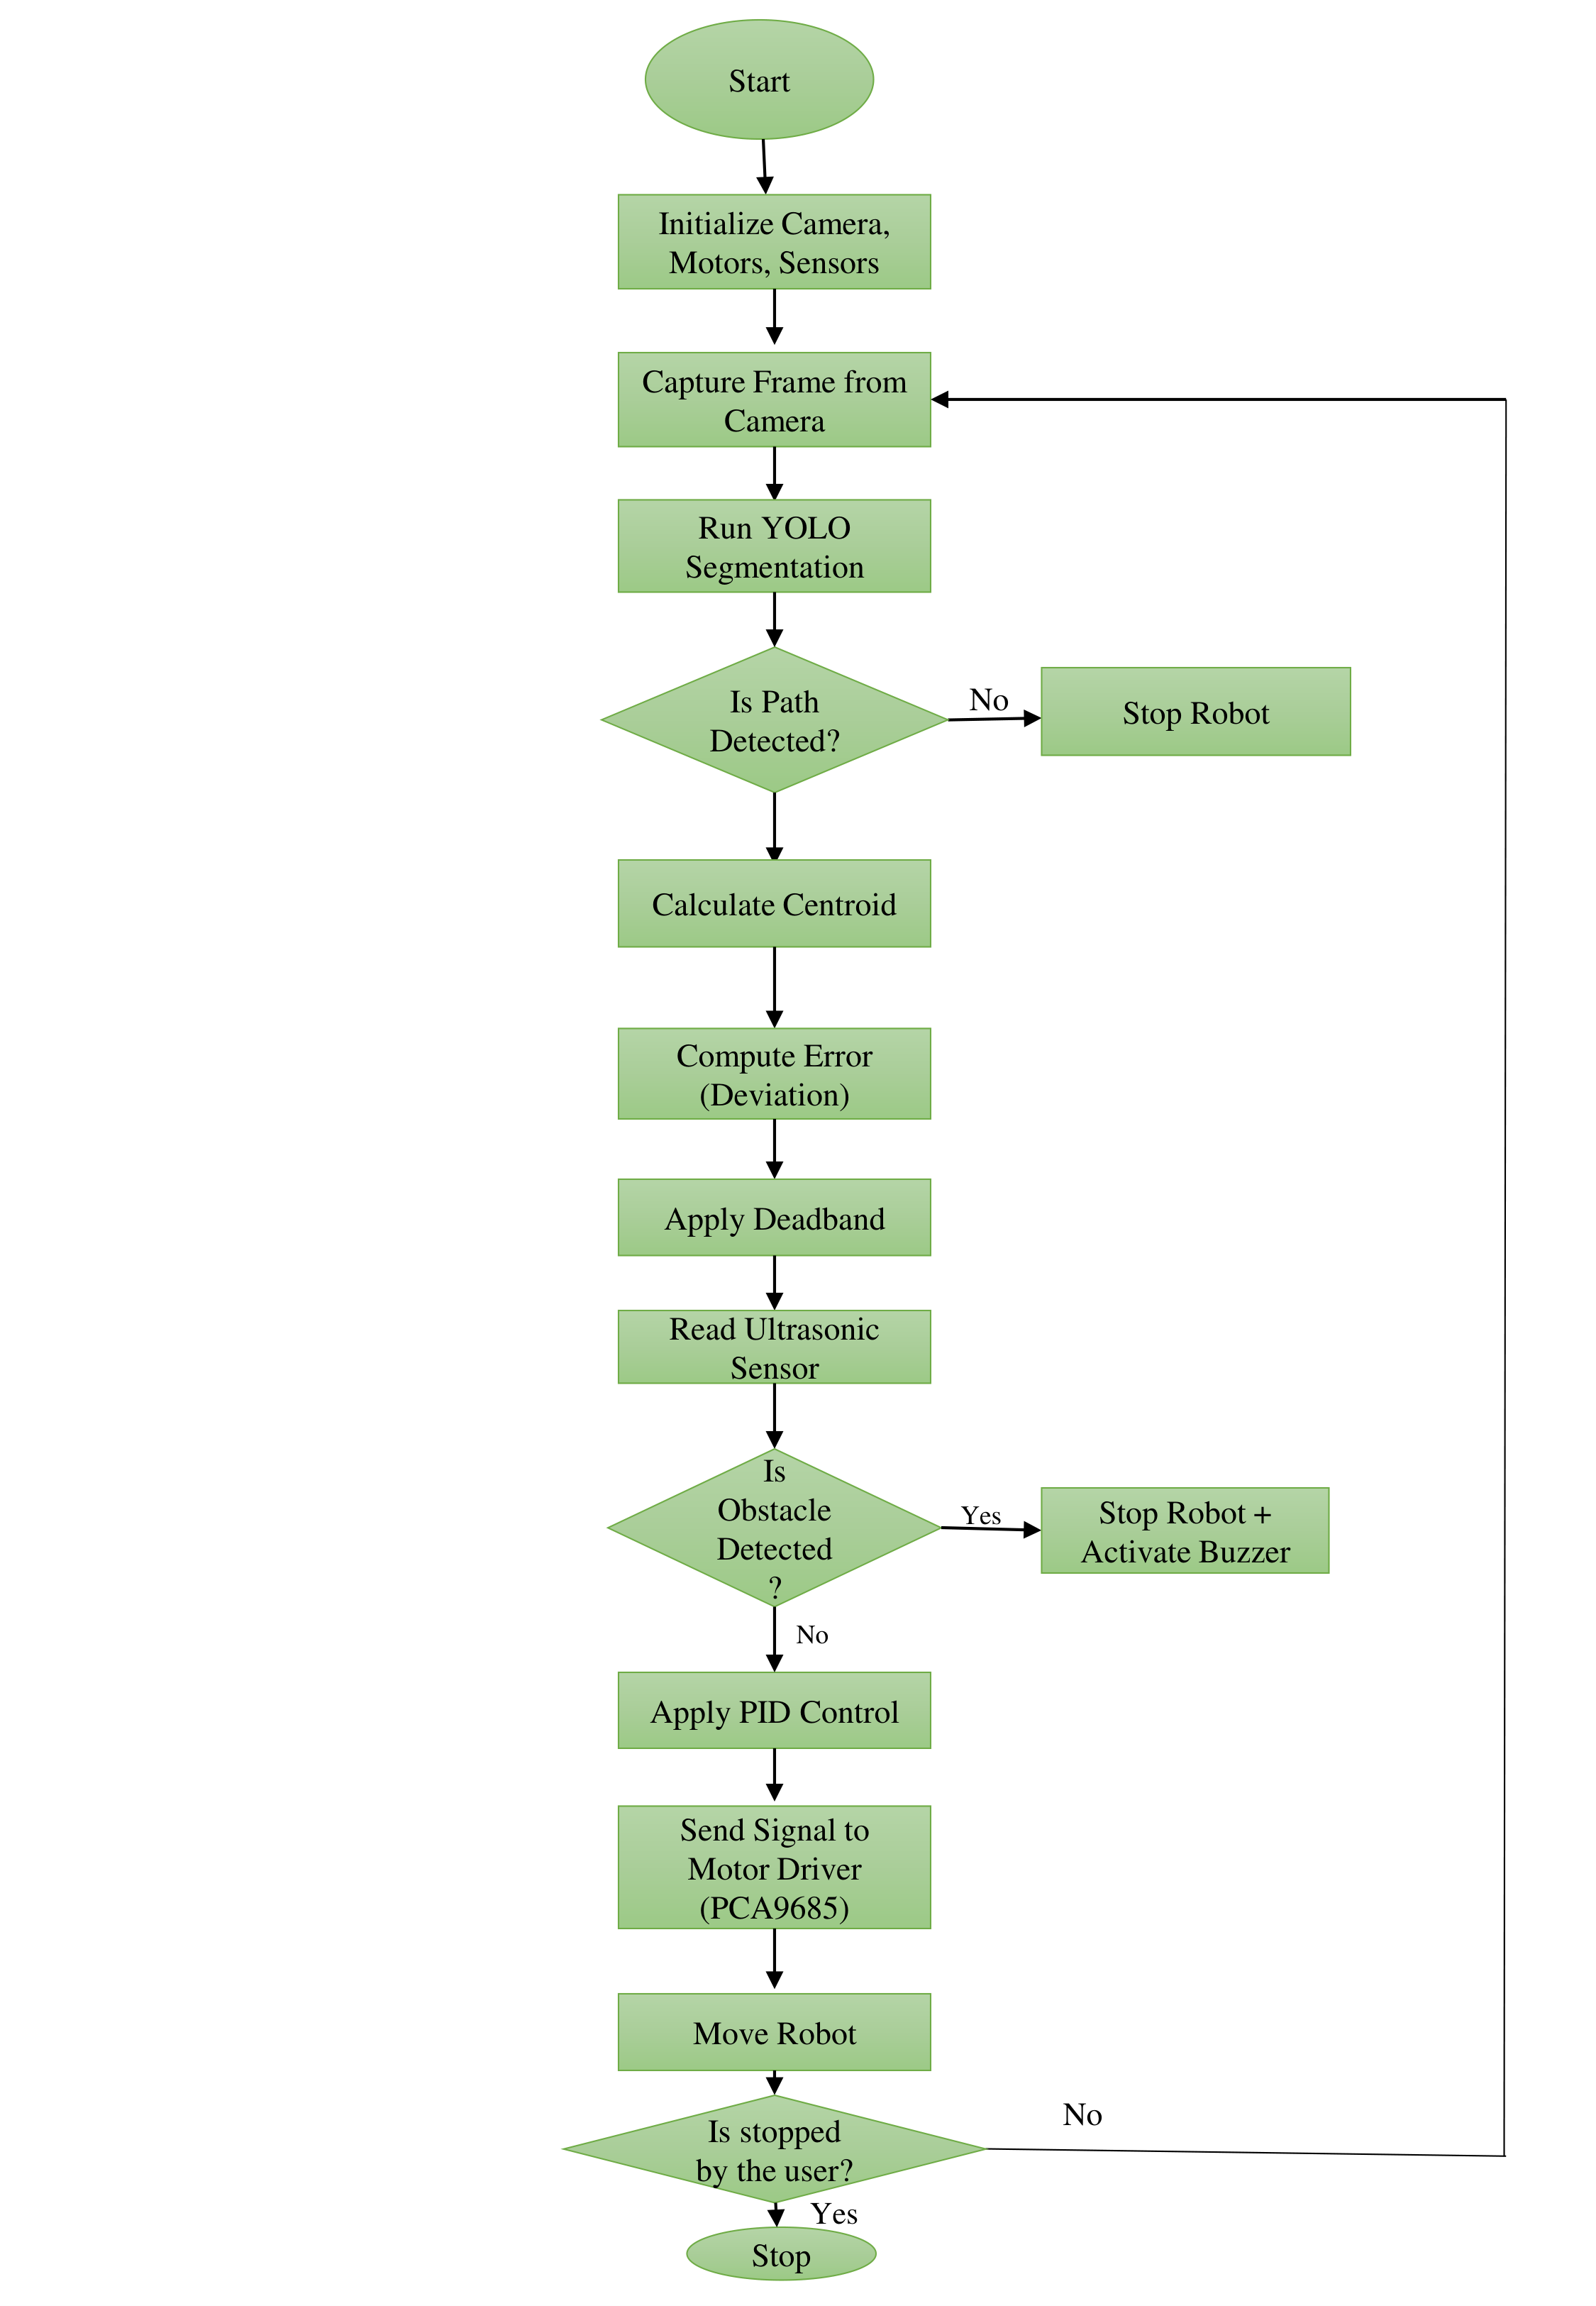
\includegraphics[height=0.88\textheight]{robot_flowchart.png}
  \caption{Step-by-step control flow of the autonomous path-following robot.}
  \label{fig:robotflow}
\end{figure}

\clearpage

\subsection{Threading Architecture}

The autonomous navigation software is structured around a four-thread
concurrent execution model \cite{r26}. Table~\ref{tab:threads}
summarises the four threads and their responsibilities.

\begin{table}[tbp]
  \centering
  \caption{Concurrent thread model of the autonomous navigation system.}
  \label{tab:threads}
  \begin{tabular}{lcc}
    \toprule
    Thread Name                          & Rate    & Responsibility \\
    \midrule
    \texttt{\_vision\_loop}              & 20\,Hz  & ONNX inference, PID control, CSV logging \\
    \texttt{\_obstacle\_detection\_loop} & 10\,Hz  & HC-SR04 polling, buzzer activation \\
    \texttt{\_movement\_loop}            & 10\,Hz  & PWM motor command execution \\
    \texttt{\_encoder\_loop}             & 100\,Hz & Speed ramp simulation \\
    \bottomrule
  \end{tabular}
\end{table}

\subsection{Vision Module and Real-Time Path Segmentation}

At each cycle of the vision loop, a 640$\times$480 pixel frame is
captured from the camera and passed to the ONNX Runtime inference
session at the fixed input resolution of 320$\times$320 pixels. The
YOLOv8n-seg model produces instance segmentation masks for the class
\texttt{path} within the bottom 30\% ROI.

Figure~\ref{fig:detect} illustrates the real-time path segmentation
output during an autonomous run. The green overlay represents the
YOLOv8 instance segmentation mask for the \texttt{path} class. The
output is produced in real time at 15.4\,FPS on the Raspberry Pi~5 CPU.

\begin{figure}[tbp]
  \centering
  \includegraphics[width=0.88\textwidth]{capture_1.jpg}
  \caption{Real-time YOLOv8n-seg path segmentation output at 15.4\,FPS on the Raspberry Pi~5 CPU. The green mask overlay covers the detected \texttt{path} class within the bottom 30\% ROI; the deviation arrow indicates the current PID steering correction direction and magnitude.}
  \label{fig:detect}
\end{figure}

During an autonomous run, the bottom 30\% region of interest is
highlighted with the YOLOv8 segmentation mask drawn in green over the
detected red-tape path. The path centroid is marked, and the deviation
arrow indicates the direction and magnitude of the current steering
correction. This overlay was visible in the live MJPEG feed on the web
dashboard throughout all 20 autonomous trials.

Within the ROI, the horizontal centroid of the detected path mask is
computed and normalised relative to the horizontal frame centre to
produce a deviation signal in the range $[-1.0,\,+1.0]$. A deadband
filter of $\pm 0.04$ is applied before the signal is passed to the
PID controller.

Algorithm~\ref{alg:vision} formalises the complete vision-based deviation computation executed at every cycle of the \texttt{\_vision\_loop} thread at 20\,Hz. The procedure begins by resizing the captured frame to $320\times320$ pixels, which matches the fixed static input shape of the deployed ONNX model. The ONNX Runtime session is then called to produce a set of instance segmentation masks $\mathcal{M}$ and their corresponding confidence scores $\mathcal{S}$. If no detection is returned, or if the highest confidence score falls below the threshold of 0.50, the function returns \texttt{None}, signalling the main loop to halt forward motion and await path reacquisition. When a valid detection is present, the mask with the highest confidence score is selected and cropped to the bottom 30\% region of interest. The centroid of the binary mask within that region is computed as a pixel-weighted mean, yielding the horizontal position $C_x$. This position is normalised to the range $[-1.0,\,+1.0]$ relative to the frame half-width, and a deadband of $\pm 0.04$ is applied to suppress spurious corrections on near-straight sections. The resulting scalar $d$ is the deviation signal consumed by the PID steering controller.

\begin{algorithm}[H]
\DontPrintSemicolon
\caption{Vision-Based Path Deviation Computation}
\label{alg:vision}
\KwIn{Camera frame $F$ at $640\times480$ resolution}
\KwOut{Normalised lateral deviation $d\in[-1.0,\,+1.0]$, or \texttt{None} if no path found}
\BlankLine
Resize $F$ to $320\times320$ pixels for ONNX Runtime input\;
$\mathcal{M},\,\mathcal{S} \leftarrow \texttt{ONNX.run}(F)$ \tcp*{instance masks and confidence scores}
\If{$|\mathcal{S}|=0$ \textbf{or} $\max(\mathcal{S})<0.50$}{
  \Return \texttt{None} \tcp*{no path detected above threshold}
}
Select best mask $M^{*} \leftarrow \mathcal{M}[\arg\max(\mathcal{S})]$\;
Define ROI as bottom 30\% of frame: rows $\lfloor 0.70H\rfloor$ to $H$\;
$M_{\text{roi}} \leftarrow M^{*}\cap\text{ROI}$\;
\If{$\sum M_{\text{roi}}=0$}{
  \Return \texttt{None} \tcp*{mask absent from ROI}
}
Compute centroid: $\displaystyle C_x = \frac{\sum_{i,j} j\cdot M_{\text{roi}}[i,j]}{\sum_{i,j} M_{\text{roi}}[i,j]}$\;
Normalise: $d \leftarrow \dfrac{C_x - W/2}{W/2}$, where $W=640$\;
Apply deadband: \textbf{if} $|d|<0.04$ \textbf{then} $d\leftarrow 0.0$\;
\Return $d$\;
\end{algorithm}

\subsection{PID Steering Controller}

The path deviation signal after deadband filtering serves as the error
input $e(t)$ to a discrete-time PID controller. Using
Equation~\eqref{eq:pid}, the control output $u(t)$ is computed as:

\begin{equation}
  u(t) = K_p \, e(t)
       + K_i \sum_{k=0}^{t} e(k)\,\Delta t
       + K_d \, \frac{e(t) - e(t-1)}{\Delta t}
  \label{eq:pid}
\end{equation}

where $u(t)$ is the steering correction applied to the motor driver
\cite{r9,r10,r11}.
The gains were tuned through iterative experimentation: $K_p = 13.2$,
$K_i = 0.0$, and $K_d = 0.475$. The proportional gain provides
immediate corrective response, the integral term was set to zero to
avoid oscillatory motion, and the derivative gain provides damping
against rapid deviation changes. PID control was selected for its
computational efficiency and demonstrated effectiveness on
differential-drive platforms \cite{r10,r9,r11}.

The controller output $u(t)$ is clamped to $[-1.0,\,+1.0]$. Differential
steering adds $u(t)$ to the right motor speed and subtracts $u(t)$
from the left motor speed. Per-wheel calibration factors from
Table~\ref{tab:motor} are applied before PWM conversion.

Algorithm~\ref{alg:pid} details the full discrete-time PID implementation including anti-windup clamping and differential motor output computation. The algorithm receives the current deviation error $e(t)$, the previous error $e(t{-}1)$, the running integral state $I$, and the fixed time step $\Delta t = 0.05$\,s corresponding to the 20\,Hz control rate. The proportional term $P$ is computed directly as $K_p \cdot e(t)$ with $K_p = 13.2$, providing an immediate corrective response proportional to the magnitude of the path deviation. The integral accumulator $I$ is updated and then clamped to $[-1.0,\,+1.0]$ to implement anti-windup protection; because $K_i = 0.0$ was found to cause oscillatory motion during empirical tuning, the integral contribution is effectively disabled. The derivative term $D$ is computed as $K_d \cdot (e(t) - e(t{-}1)) / \Delta t$ with $K_d = 0.475$, providing damping against rapid changes in deviation such as those encountered at tight corners. The combined output $u(t)$ is clamped to $[-1.0,\,+1.0]$ before being applied as a differential speed offset to the left and right motor channels.

\begin{algorithm}[H]
\DontPrintSemicolon
\caption{Discrete-Time PID Steering Controller with Anti-Windup}
\label{alg:pid}
\KwIn{Error $e(t)$, previous error $e(t{-}1)$, integral state $I$, time step $\Delta t=0.05$\,s}
\KwOut{Steering correction $u(t)\in[-1.0,\,+1.0]$, updated integral $I$}
\BlankLine
$P \leftarrow K_p \cdot e(t)$ \tcp*{proportional: $K_p=13.2$}
$I \leftarrow I + e(t)\cdot\Delta t$\;
$I \leftarrow \operatorname{clamp}(I,\;{-}1.0,\;{+}1.0)$ \tcp*{anti-windup; $K_i=0.0$}
$D \leftarrow K_d\cdot\dfrac{e(t)-e(t{-}1)}{\Delta t}$ \tcp*{derivative: $K_d=0.475$}
$u(t) \leftarrow P + K_i\cdot I + D$\;
$u(t) \leftarrow \operatorname{clamp}(u(t),\;{-}1.0,\;{+}1.0)$\;
\BlankLine
\tcp{Differential steering outputs (before per-wheel calibration)}
$v_R \leftarrow \operatorname{clamp}(v_{\text{base}}+u(t),\;0.0,\;1.0)$\;
$v_L \leftarrow \operatorname{clamp}(v_{\text{base}}-u(t),\;0.0,\;1.0)$\;
Apply per-wheel calibration factors from Table~\ref{tab:motor} to $v_R$, $v_L$\;
\Return $u(t)$, $I$\;
\end{algorithm}

\subsection{Safety Hierarchy}

A priority-ordered safety hierarchy governs robot state at every
control cycle. First, if the HC-SR04 sensor measures below 20\,cm,
all motors stop and the buzzer activates. Second, if YOLOv8 detects
no path within the ROI, all motors stop and the system waits for
reacquisition. Third, if both conditions are clear, PID steering is
applied and the robot moves forward.

Algorithm~\ref{alg:navloop} presents the complete main control loop of the autonomous navigation system, integrating the threading model, safety hierarchy, vision pipeline (Algorithm~\ref{alg:vision}), and PID steering (Algorithm~\ref{alg:pid}). Upon receiving a START command from the web dashboard, the system initialises the camera stream, the PCA9685 PWM driver, and the GPIO pins, then opens a new auto-incremented CSV log file. Four daemon threads are spawned concurrently: the \texttt{\_vision\_loop} at 20\,Hz, the \texttt{\_obstacle\_loop} at 10\,Hz, the \texttt{\_movement\_loop} at 10\,Hz, and the \texttt{\_encoder\_loop} at 100\,Hz. Within the main while loop, the highest-priority check is the obstacle distance measurement: if $d_{\text{obs}} < 20$\,cm, all motors are stopped immediately and the buzzer is activated, bypassing the vision and PID stages entirely. If the path is clear, a camera frame is captured and passed to Algorithm~\ref{alg:vision} to obtain the deviation signal $d$. If the vision module returns \texttt{None}, all motors are halted to await path reacquisition. Otherwise, Algorithm~\ref{alg:pid} computes the steering correction $u(t)$, which is dispatched to the motor driver and logged to the CSV file together with all 16 telemetry fields. The loop continues until a STOP command is received, at which point all motors are set to neutral and the log file is closed.

\begin{algorithm}[H]
\DontPrintSemicolon
\caption{Autonomous Navigation Main Control Loop}
\label{alg:navloop}
\KwIn{START command issued from web dashboard}
\KwOut{Trajectory CSV log file with 16 fields per record}
\BlankLine
Initialise camera (\texttt{cv2.VideoCapture}), PCA9685 PWM driver, GPIO\;
Initialise CSV logger with auto-incremented filename\;
$e_{\text{prev}}\leftarrow 0$;\quad $I\leftarrow 0$;\quad $\textit{running}\leftarrow\texttt{True}$\;
Spawn daemon threads: \texttt{\_vision\_loop} (20\,Hz), \texttt{\_obstacle\_loop} (10\,Hz), \texttt{\_movement\_loop} (10\,Hz), \texttt{\_encoder\_loop} (100\,Hz)\;
\BlankLine
\While{$\textit{running}$}{
  \If{STOP command received}{
    $\textit{running}\leftarrow\texttt{False}$\; \textbf{break}\;
  }
  \BlankLine
  \tcp{Safety check: obstacle}
  $d_{\text{obs}}\leftarrow\texttt{HC\_SR04.measure()}$\;
  \If{$d_{\text{obs}}<20\,\text{cm}$}{
    \texttt{StopAllMotors()}\; \texttt{Buzzer.on()}\; \textbf{continue}\;
  }
  \BlankLine
  \tcp{Vision: capture and segment}
  $F \leftarrow \texttt{Camera.read()}$\;
  $d \leftarrow \texttt{VisionDeviation}(F)$ \tcp*{Algorithm~\ref{alg:vision}}
  \If{$d=\texttt{None}$}{
    \texttt{StopAllMotors()}\; \textbf{continue} \tcp*{await path reacquisition}
  }
  \BlankLine
  \tcp{PID steering and logging}
  $u(t),\,I \leftarrow \texttt{PIDControl}(d,\,e_{\text{prev}},\,I,\,\Delta t)$ \tcp*{Algorithm~\ref{alg:pid}}
  $e_{\text{prev}}\leftarrow d$\;
  \texttt{SendMotorCommand}$(u(t))$\;
  \texttt{CSVLogger.write}(timestamp, frameID, $d$, $u(t)$, $d_{\text{obs}}$, conf, $\ldots$)\;
}
\BlankLine
\texttt{StopAllMotors()}\; \texttt{Camera.release()}\; \Return CSV log\;
\end{algorithm}

\subsection{Trajectory Logging System and CSV Data Collection}

A structured comma-separated values (CSV) logging system records the complete
state of the robot at every iteration of the vision loop running at 20\,Hz.
Each log record contains 16 fields: a UTC timestamp, a sequential frame
identifier, the raw lateral deviation signal, the deadband-filtered deviation,
the proportional term, the integral term, the derivative term, the PID steering output, the left motor speed command, the right
motor speed command, the ultrasonic obstacle distance, the path detection
confidence score, the detected path centroid pixel coordinates ($C_x$, $C_y$),
the estimated robot position offset, and the current control state string
(\texttt{FORWARD}, \texttt{OBSTACLE}, or \texttt{NO PATH}).

CSV files were collected as follows. At the start of each autonomous trial,
the operator issued a START command through the web dashboard, which triggered
the initialisation of a new log file with an auto-incremented filename of the
form \texttt{run\_001.csv}, \texttt{run\_002.csv}, and so on, stored on the
Raspberry Pi~5 local filesystem under the \texttt{logs/} directory. The vision
loop then ran continuously at 20\,Hz, appending one record to the active CSV
file at every cycle. At the end of each trial, the operator issued a STOP
command, which flushed and closed the file before setting all motor channels
to neutral. A total of 20 autonomous trials were conducted across the three
path geometry categories (straight, curved, and mixed-turn), yielding 20
individual CSV log files. These files were subsequently transferred from the
Raspberry Pi~5 to a host workstation over Secure Shell (SSH) for offline
analysis. The log files were used to compute all navigation performance metrics
reported in Chapter~4, including mean absolute deviation, maximum deviation,
steer magnitude, and path-recovery counts.

\subsection{Robot Position Estimation}

During experimental trials, the robot's lateral position relative to the
centre of the red tape path was estimated using a colour-marker-based method
applied to the downward-facing camera image. A small square of blue adhesive
tape was affixed to the top surface of the robot chassis, directly above the
camera mount, serving as the robot's reference marker. The blue colour was
chosen because it provides the highest chrominance contrast against both the
red tape path and the typical beige or grey tiled floor surfaces found in the
laboratory.

At each video frame, the position of the robot reference marker was located
by applying a blue-colour threshold in the Hue-Saturation-Value colour space
to isolate the blue tape region and computing its centroid, denoted
$(B_x,\,B_y)$, in pixel coordinates. Simultaneously, the centroid of the
detected red tape path mask within the region of interest, denoted
$(R_x,\,R_y)$, was obtained from the You Only Look Once segmentation
inference output as described in Section~3.3.3. The robot's position
relative to the path centre was then expressed as the Euclidean distance
between these two centroids:

\begin{equation}
  d_{\text{pos}} = \sqrt{(R_x - B_x)^2 + (R_y - B_y)^2}
  \label{eq:euclidean}
\end{equation}

\noindent
where $d_{\text{pos}}$ is the pixel-domain position offset between the robot
marker and the path centre \cite{r5,r6,r8}. A value of $d_{\text{pos}} = 0$ would indicate
that the robot reference marker is exactly centred over the detected path.
In practice, the closed-loop PID controller
acted to minimise the lateral component of this offset, driving the robot
toward a state in which the horizontal coordinates $B_x$ and $R_x$ converge.
The vertical component $(R_y - B_y)$ reflects the forward distance between
the camera viewpoint and the path region below, which remains approximately
constant during straight running and increases slightly during turns.

This distance measure was logged as the \texttt{robot\_position\_offset} field
in each CSV record, providing a frame-by-frame ground-truth estimate of
positional accuracy independent of the deviation signal computed by the
PID controller. The field was used during
post-run analysis to verify that the deviation signal faithfully represented
the actual robot-to-path alignment, confirming the validity of using lateral
normalised deviation as the primary performance metric in Chapter~4.

\subsection{Web Monitoring Dashboard}

A Flask-based web dashboard at \texttt{http://<Pi-IP>:5000} provides
real-time monitoring. A live MJPEG video feed at \texttt{/video\_feed}
overlays the YOLOv8 segmentation mask, ROI boundary, path centreline,
and deviation arrow at 20\,Hz. Status fields are polled every 500\,ms
from the \texttt{/api/status} endpoint.

\section{Environmental Monitoring System}

\subsection{Data Flow Overview}

The data flow of the complete environmental monitoring subsystem is
illustrated in Figure~\ref{fig:envflow}. The flowchart describes the
full pipeline from serial communication initialisation through sensor
data acquisition, validity checking, data processing, and the four
parallel output operations.

\textbf{Step 1: Start.} Executing \texttt{main.py} on the Raspberry Pi~3
initialises the SQLite schema and launches the serial reader thread.

\textbf{Step 2: Initialise Serial Communication.} The serial reader
opens the USB connection to the Arduino UNO at \texttt{/dev/ttyACM0}
and 9600 baud using PySerial \cite{r44}.

\textbf{Step 3: Read Sensor Data.} The Arduino reads the DHT11 and
MQ135 sensors and transmits the formatted string
\texttt{T:28.0,H:38.0,AQ:68} over the serial connection.

\textbf{Step 4: Is Data Valid?} The Raspberry Pi~3 parses and validates
the received string. Invalid readings are discarded.

\textbf{Step 5: Process Data.} Valid readings are passed through the
AQ-to-CO$_2$ calibration formula given in Equation~\eqref{eq:co2},
and the alert decision logic is applied.

\textbf{Step 6: Four Parallel Output Operations.} After processing,
the reading is simultaneously dispatched to: (a) SQLite local storage,
(b) Firebase Realtime Database cloud push, (c) ThingSpeak IoT channel
transmission, and (d) Flask live dashboard update via HTTP.

\textbf{Step 7: Wait 15 Seconds.} The system waits 15 seconds to
enforce the ThingSpeak free-tier minimum update interval.

\textbf{Step 8: Is Stopped by User?} If a stop command has been issued,
the loop terminates; otherwise the flow returns to Step 3.

\begin{figure}[p]
  \centering
  \makebox[\textwidth][c]{%
    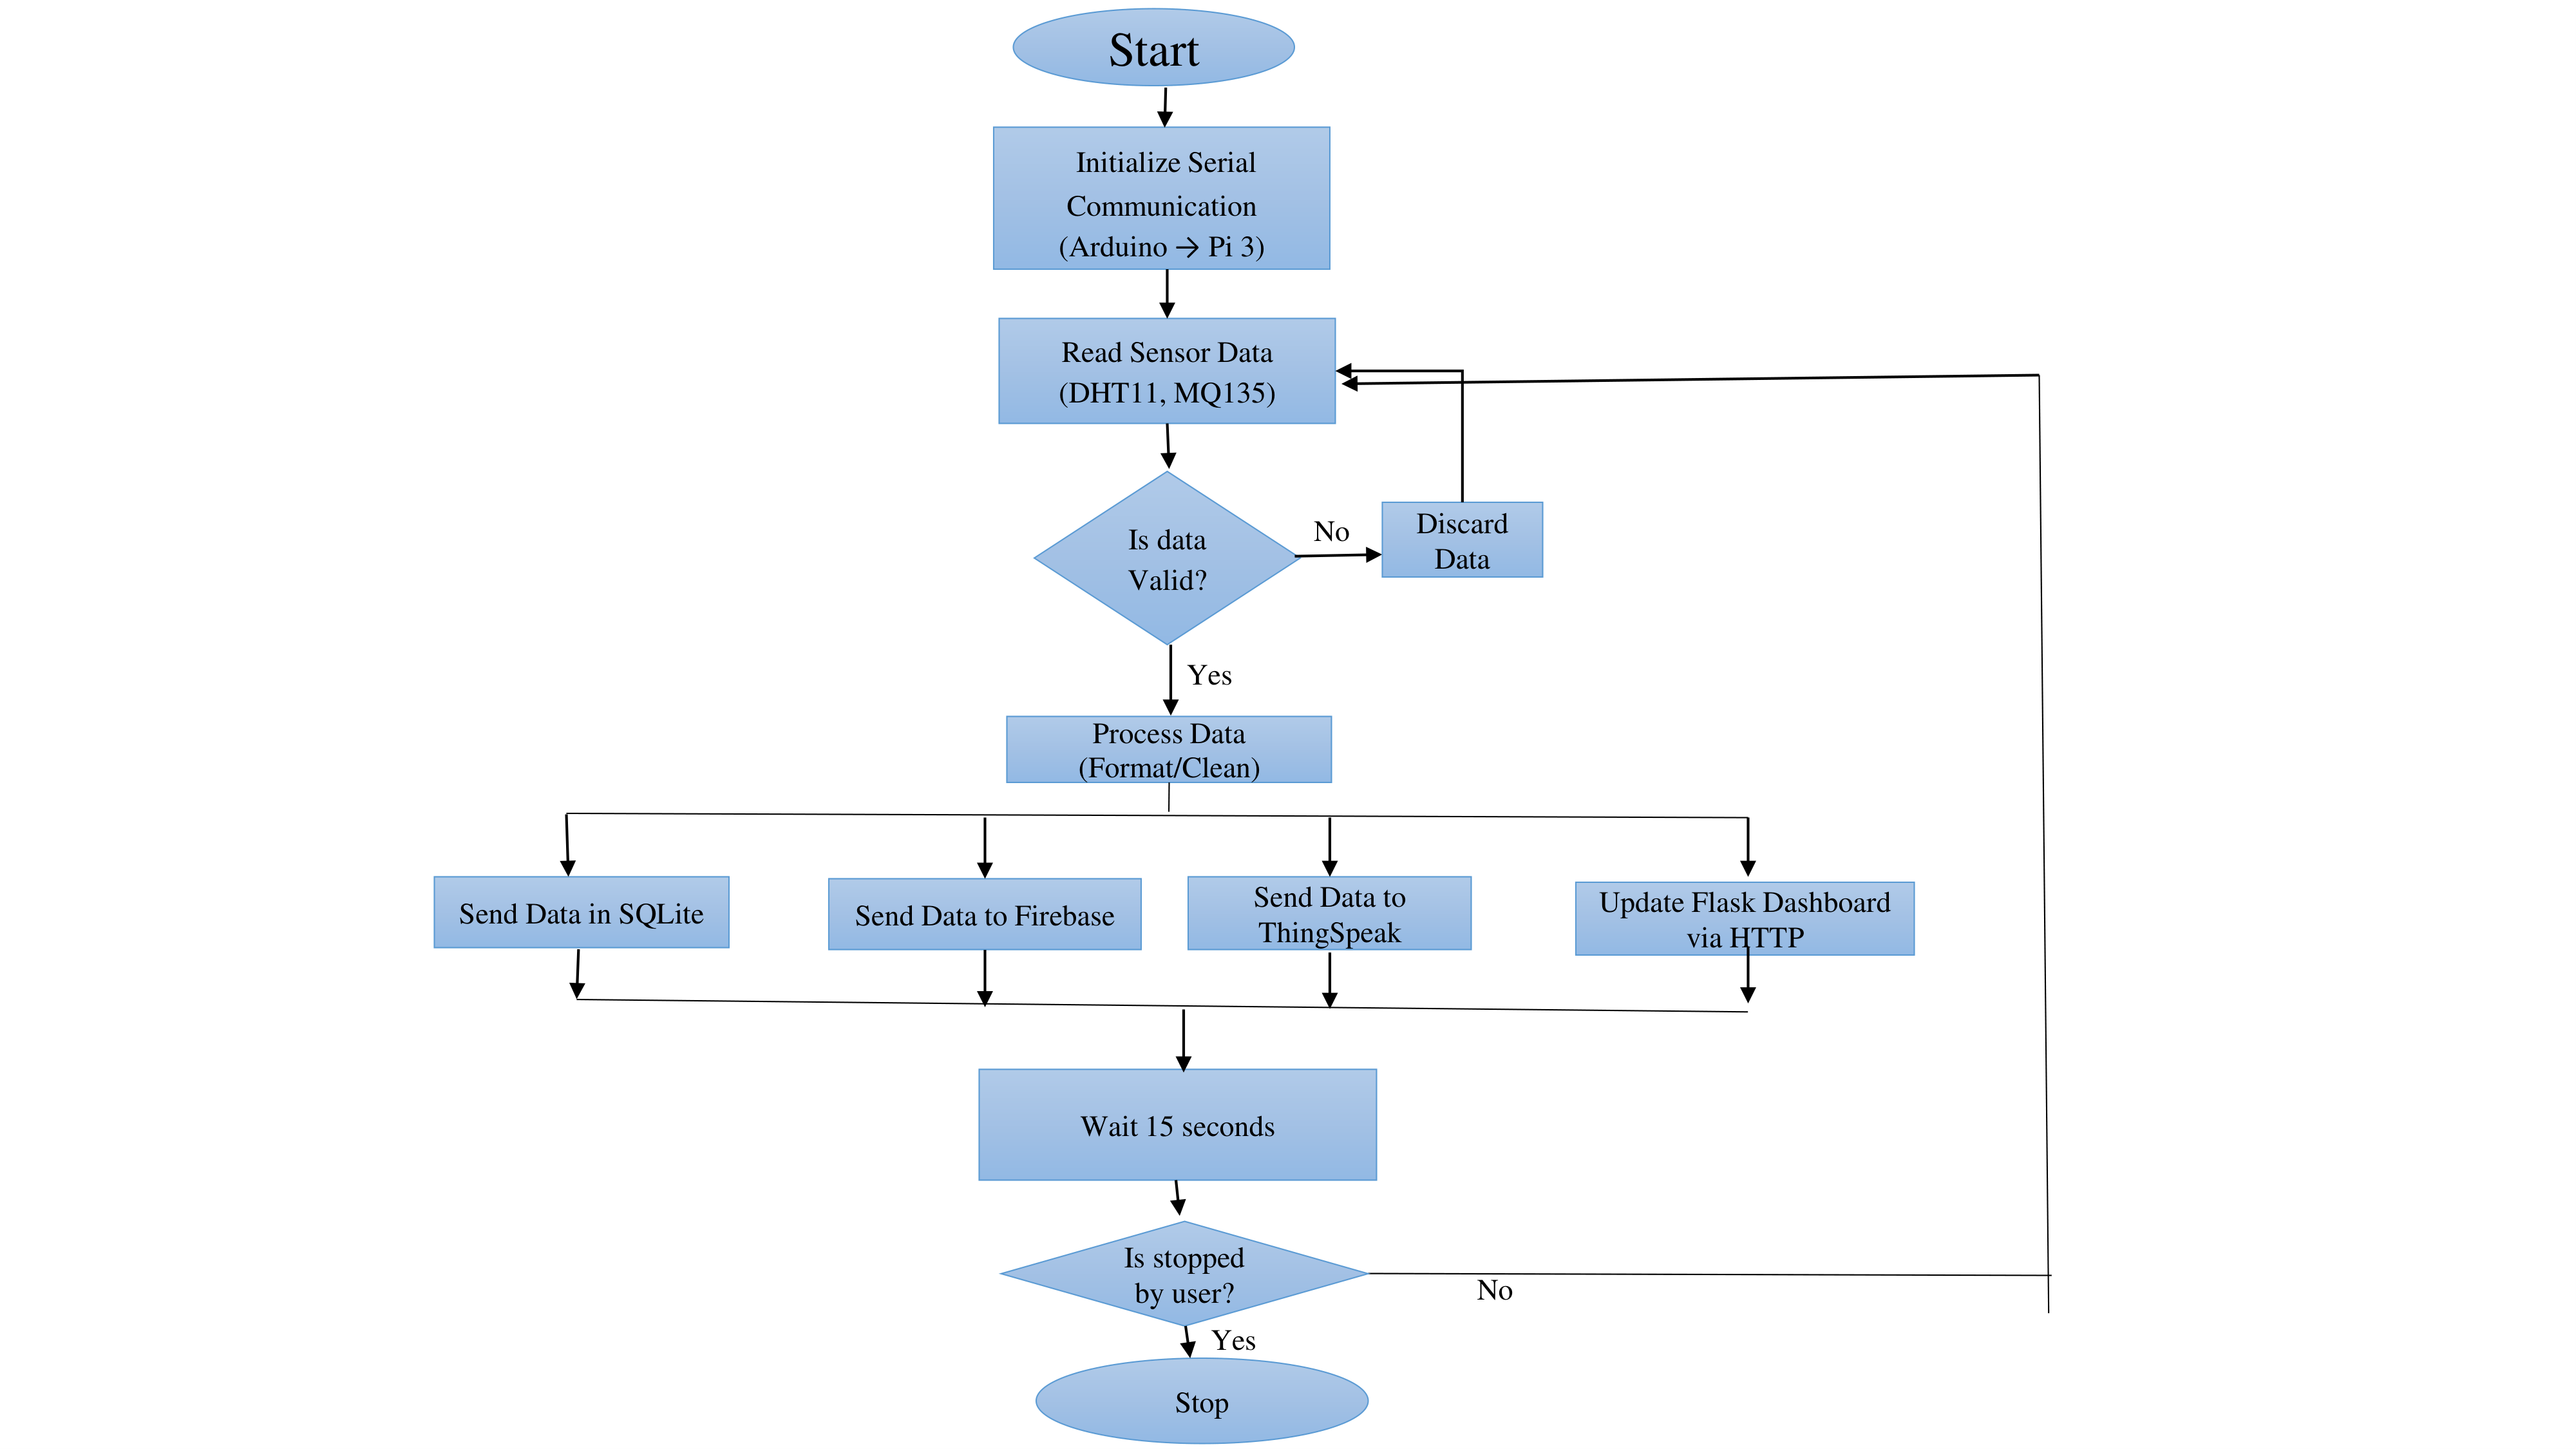
\includegraphics[
      width=1.3\textwidth,
      height=0.95\textheight,
      keepaspectratio
    ]{env_flowchart.png}%
  }
  \caption{Data flow of the environmental monitoring subsystem from sensor acquisition to cloud storage.}
  \label{fig:envflow}
\end{figure}

\subsection{Sensor Hardware and Integration}

The DHT11 temperature and humidity sensor measures ambient
temperature with accuracy $\pm 2\,^\circ$C and relative humidity with
accuracy $\pm 5\%$\,RH using a single-wire serial data protocol.

The MQ135 air quality gas sensor detects CO$_2$, ammonia,
benzene, and alcohol vapours through an electrochemical sensing element,
producing an analogue output voltage read by the Arduino UNO ADC as a
raw integer in the range 0 to 1023.

The Arduino UNO microcontroller reads both sensors at regular
intervals and transmits formatted serial strings at 9600 baud.

\subsection{Arduino Sensor Firmware}

The Arduino UNO firmware manages all sensor-level acquisition in the
environmental monitoring subsystem. The firmware is built around a simple
polling loop executing at a 5-second interval, matching the Raspberry Pi~3
processing rate and the ThingSpeak free-tier rate-limiting constraint.

The DHT11 sensor is interfaced through the \texttt{DHT} Arduino library.
Raw temperature ($T$) and humidity ($H$) values are validated against the
sensor's safe operating bounds before transmission:
$0^\circ\text{C}\le T\le 50^\circ\text{C}$ and
$20\,\%\text{RH}\le H\le 90\,\%\text{RH}$. If either value is
out-of-range or the DHT11 returns a NaN reading, the firmware transmits
an error marker and retries on the next cycle without corrupting the
Raspberry Pi~3 parser state.

The MQ135 sensor is sampled through \texttt{analogRead(A0)}, which
returns a 10-bit ADC integer in the range $[0,\,1023]$. No calibration
is performed on the Arduino; all calibration and classification logic
resides on the Raspberry Pi~3. This separation keeps the firmware simple
and the calibration parameters easy to update over SSH without
reflashing the microcontroller.

The formatted output follows the pattern
\texttt{T:\,<value>,H:\,<value>,AQ:\,<value>\textbackslash n}
transmitted at 9600\,baud. The Raspberry Pi~3 reads one line per
acquisition cycle, strips whitespace, splits on commas, and extracts the
three field values for the calibration pipeline.

Algorithm~\ref{alg:arduino} formalises the Arduino firmware state machine including warm-up, validation, and serial transmission. On power-on, the firmware initialises the DHT11 sensor on digital pin 2, configures the MQ135 analogue input on pin A0, and opens the serial port at 9600\,baud. A mandatory 2-second warm-up delay is imposed to allow the DHT11 to stabilise before the first reading is taken. The main acquisition loop then executes at a fixed 5-second interval. At each iteration, the firmware reads the temperature $T$ and humidity $H$ values from the DHT11 library and reads the 10-bit ADC value from the MQ135 sensor. Before transmitting any data, two validation checks are applied: if either $T$ or $H$ is not a number (\texttt{NaN}), an \texttt{ERROR:DHT\_FAULT} message is transmitted and the cycle is skipped; if either value falls outside the sensor's operating bounds ($0\le T\le 50\,^\circ$C and $20\le H\le 90$\,\%RH), an \texttt{ERROR:OUT\_OF\_RANGE} message is transmitted and the cycle is skipped. Only when both checks pass is the formatted string \texttt{T:\!<value>,H:\!<value>,AQ:\!<value>} transmitted over the serial connection to the Raspberry Pi~3 for calibration and classification.

\begin{algorithm}[H]
\DontPrintSemicolon
\caption{Arduino UNO Sensor Acquisition Firmware}
\label{alg:arduino}
\KwIn{DHT11 and MQ135 sensor signals}
\KwOut{Formatted serial string to Raspberry Pi~3 at 9600\,baud}
\BlankLine
\tcp{Setup (executes once on power-on)}
Initialise DHT11 on digital pin 2\;
Set MQ135 analogue input to pin A0\;
Configure serial port at 9600\,baud\;
$\texttt{delay}(2000\,\text{ms})$ \tcp*{sensor warm-up period}
\BlankLine
\tcp{Acquisition loop}
\While{powered}{
  $T\leftarrow\texttt{dht.readTemperature()}$\;
  $H\leftarrow\texttt{dht.readHumidity()}$\;
  $\text{AQ}\leftarrow\texttt{analogRead(A0)}$\;
  \BlankLine
  \If{$\texttt{isnan}(T)$ \textbf{or} $\texttt{isnan}(H)$}{
    $\texttt{Serial.println("ERROR:DHT\_FAULT")}$\; \textbf{continue}\;
  }
  \If{$T<0$ \textbf{or} $T>50$ \textbf{or} $H<20$ \textbf{or} $H>90$}{
    $\texttt{Serial.println("ERROR:OUT\_OF\_RANGE")}$\; \textbf{continue}\;
  }
  \BlankLine
  $\text{msg}\leftarrow\texttt{"T:"}+T+\texttt{",H:"}+H+\texttt{",AQ:"}+\text{AQ}$\;
  $\texttt{Serial.println}(\text{msg})$ \tcp*{transmit to Raspberry Pi~3}
  $\texttt{delay}(5000\,\text{ms})$ \tcp*{5-second acquisition interval}
}
\end{algorithm}

The \textbf{Raspberry Pi~3} receives and parses the serial stream,
performs calibration, executes the alert logic, and manages all four
output channels.

\subsection{AQ-to-CO$_2$ Calibration}

The MQ135 sensor outputs a raw ADC value proportional to aggregate
gas concentration rather than a direct CO$_2$ reading. A linear
interpolation formula, based on the MQ135 sensor characterisation
described in \cite{r50,r1,r2}, maps this raw value to an estimated
CO$_2$ concentration in parts per million (Equation~\eqref{eq:co2}):

\begin{equation}
  \text{CO}_2\,(\text{ppm}) = \text{CO}_{2,\min}
  + \frac{(\text{AQ}_\text{raw} - \text{AQ}_\text{clean})}
         {(\text{AQ}_\text{max} - \text{AQ}_\text{clean})}
  \times (\text{CO}_{2,\max} - \text{CO}_{2,\min})
  \label{eq:co2}
\end{equation}

The calibration constants are: $\text{AQ}_\text{clean} = 38$ (sensor
reading in fresh outdoor air after a 24-hour warm-up period),
$\text{AQ}_\text{max} = 650$, $\text{CO}_{2,\min} = 350\,\text{ppm}$
(typical ambient outdoor concentration), and
$\text{CO}_{2,\max} = 2500\,\text{ppm}$. The computed value is clamped
to the range $[350,\,2500]$\,ppm \cite{r50,r1,r2}.

\subsection{Data Processing and Alert Logic}

After calibration, each reading is passed through a sensor fault
validation check and then classified using a six-level priority-ordered
alert hierarchy. The classification thresholds are grounded in
established indoor air quality standards. ASHRAE Standard~62.1
\cite{r46} specifies that CO$_2$ in occupied indoor spaces should not
exceed approximately 1100\,ppm (700\,ppm above the outdoor ambient
concentration of $\sim$400\,ppm). The WHO Indoor Air Quality Guidelines
\cite{r47} and supporting epidemiological research \cite{r48,r49}
indicate that CO$_2$ concentrations above 1000\,ppm are associated with
noticeably reduced air quality and early health effects, while levels
above 2000\,ppm are considered poor and require immediate action.

Table~\ref{tab:alertlevels} summarises the CO$_2$ thresholds and
corresponding alert levels implemented in the system.

\begin{table}[tbp]
  \centering
  \caption{CO$_2$ concentration thresholds and alert classifications.}
  \label{tab:alertlevels}
  \begin{tabular}{lll}
    \toprule
    Alert Level    & CO$_2$ Range (ppm)  & Action \\
    \midrule
    OK             & $< 600$             & Conditions nominal; no action needed \\
    VENTILATION    & $600$--$1000$       & Air quality declining; increase ventilation \\
    WARNING        & $1000$--$1500$      & Elevated CO$_2$; monitor closely \\
    CRITICAL       & $1500$--$2000$      & Hazardous classification; ventilate immediately \\
    CRITICAL+      & $> 2000$            & Severe; possible gas leak or equipment fault \\
    HARDWARE       & Any                 & Sensor fault; temperature or humidity out of range \\
    \bottomrule
  \end{tabular}
\end{table}

The six-level classification hierarchy, in descending priority order, is:

\begin{enumerate}
  \item \textbf{HARDWARE:} The DHT11 returned a value outside its
        valid range, indicating a sensor fault or wiring issue.
  \item \textbf{CRITICAL+:} CO$_2$ exceeds 2000\,ppm; severe
        conditions requiring immediate action \cite{r47,r48}.
  \item \textbf{CRITICAL:} CO$_2$ in the 1500--2000\,ppm range;
        ventilate the space immediately \cite{r47}.
  \item \textbf{WARNING:} CO$_2$ in the 1000--1500\,ppm range;
        air quality is declining and should be monitored \cite{r48,r49}.
  \item \textbf{VENTILATION:} CO$_2$ in the 600--1000\,ppm range;
        increase ventilation to prevent further rise \cite{r46}.
  \item \textbf{OK:} All sensor values within nominal ranges and
        CO$_2$ below 600\,ppm.
\end{enumerate}

Algorithm~\ref{alg:envpipeline} formalises the complete data acquisition and dispatch pipeline executed on the Raspberry Pi~3. The pipeline begins by initialising the SQLite database schema and opening the serial connection to the Arduino UNO at \texttt{/dev/ttyACM0} at 9600\,baud. A background Flask server is launched on \texttt{0.0.0.0:5000} to serve the live dashboard. Within the main acquisition loop, each line received from the serial port is checked for the expected \texttt{T:} prefix; malformed or error lines are discarded without disrupting the loop. Valid lines are parsed to extract $T$, $H$, and the raw AQ value. If the sensor values are out of range, the alert level is immediately set to \texttt{HARDWARE}. Otherwise, the raw AQ value is converted to an estimated CO$_2$ concentration using Equation~\eqref{eq:co2}, and the resulting value is passed to the six-level classification logic. After classification, the processed reading is dispatched simultaneously to four output channels: SQLite local storage, the Firebase Realtime Database cloud node, the ThingSpeak IoT platform (subject to the 15-second rate-limiting guard), and the Flask dashboard state. The loop then waits 15\,s before the next acquisition cycle.

Algorithm~\ref{alg:alert} details the six-level priority-ordered alert classification applied to every processed CO$_2$ reading. The classification is performed in strict priority order from the most severe condition to the most benign. The highest priority level, \texttt{HARDWARE}, is triggered when the sensor fault flag $f = 1$, indicating that the DHT11 reported an out-of-range or \texttt{NaN} reading in the current cycle. If no hardware fault is present, the CO$_2$ concentration is compared against four descending thresholds: \texttt{CRITICAL+} for values above 2000\,ppm \cite{r47,r48}, \texttt{CRITICAL} for values between 1500 and 2000\,ppm \cite{r47}, \texttt{WARNING} for values between 1000 and 1500\,ppm \cite{r48,r49}, and \texttt{VENTILATION} for values between 600 and 1000\,ppm \cite{r46}. If none of these thresholds are exceeded, the reading is classified as \texttt{OK}, indicating that all sensor values are within their nominal operating ranges.

\begin{algorithm}[H]
\DontPrintSemicolon
\caption{Environmental Monitoring Acquisition and Dispatch Pipeline}
\label{alg:envpipeline}
\KwIn{Serial stream from Arduino UNO}
\KwOut{Readings persisted to SQLite, Firebase, ThingSpeak, and Flask}
\BlankLine
Initialise SQLite schema via \texttt{init\_db()}\;
Open serial port \texttt{/dev/ttyACM0} at 9600\,baud (PySerial)\;
Start Flask server on \texttt{0.0.0.0:5000} in background thread\;
\BlankLine
\While{not stopped}{
  $\text{line}\leftarrow\texttt{serial.readline().decode().strip()}$\;
  \If{not $\text{line.startswith("T:")}$}{
    \textbf{continue} \tcp*{discard malformed or error lines}
  }
  Parse: $T,\,H,\,\text{AQ}\leftarrow\texttt{parse}(\text{line})$\;
  \BlankLine
  \If{$T<0$ \textbf{or} $T>50$ \textbf{or} $H<20$ \textbf{or} $H>90$}{
    $\text{alert}\leftarrow\texttt{HARDWARE}$\;
  }\Else{
    $\text{CO}_2\leftarrow\texttt{calibrate}(\text{AQ})$ \tcp*{Equation~\ref{eq:co2}}
    $\text{alert}\leftarrow\texttt{ClassifyAlert}(\text{CO}_2)$ \tcp*{Algorithm~\ref{alg:alert}}
  }
  \BlankLine
  \tcp{Parallel four-channel dispatch}
  \texttt{SQLiteWrite}$(T,\,H,\,\text{AQ},\,\text{CO}_2,\,\text{alert})$\;
  \texttt{FirebasePush}$(T,\,H,\,\text{AQ},\,\text{CO}_2,\,\text{alert})$ \tcp*{daemon thread; non-blocking}
  \If{$\Delta t_{\text{ThingSpeak}}\geq 15\,\text{s}$}{
    \texttt{ThingSpeakSend}$(T,\,H,\,\text{CO}_2,\,\text{AQ})$\;
  }
  \texttt{FlaskUpdate}$\text{(latest\_reading)}$\;
  $\texttt{sleep}(15\,\text{s})$ \tcp*{rate-limiter guard}
}
\end{algorithm}

\begin{algorithm}[H]
\DontPrintSemicolon
\caption{Six-Level CO$_2$ Alert Classification (Priority-Ordered)}
\label{alg:alert}
\KwIn{$\text{CO}_2$ concentration (ppm), sensor fault flag $f\in\{0,1\}$}
\KwOut{Alert level string}
\BlankLine
\If{$f=1$}{
  \Return \texttt{HARDWARE} \tcp*{sensor fault or out-of-range reading}
}
\If{$\text{CO}_2>2000$}{
  \Return \texttt{CRITICAL+} \tcp*{severe \cite{r47,r48}}
}
\If{$1500<\text{CO}_2\leq 2000$}{
  \Return \texttt{CRITICAL} \tcp*{ventilate immediately \cite{r47}}
}
\If{$1000<\text{CO}_2\leq 1500$}{
  \Return \texttt{WARNING} \tcp*{monitor closely \cite{r48,r49}}
}
\If{$600<\text{CO}_2\leq 1000$}{
  \Return \texttt{VENTILATION} \tcp*{increase ventilation \cite{r46}}
}
\Return \texttt{OK} \tcp*{all readings nominal}
\end{algorithm}



\subsection{Multi-Channel Data Storage and Cloud Transmission}

Each processed reading is written to four parallel output channels
concurrently, as shown in Figure~\ref{fig:envflow}.

\textbf{SQLite Local Storage} writes each reading to a
\texttt{readings} table containing 14 fields. All Flask dashboard
queries are served from SQLite to ensure responsiveness independent
of cloud connectivity \cite{r23}.

\textbf{Firebase Realtime Database} \cite{r35} receives each reading
via the \texttt{firebase\_admin} Python SDK \cite{r45}, pushed to the
\texttt{/readings} node in a daemon background thread to ensure that
network timeouts never block the acquisition loop \cite{r2}.

\textbf{ThingSpeak IoT Platform} \cite{r36} receives sensor readings
via HTTP GET with six field mappings for temperature, humidity,
CO$_2$~ppm, raw AQ, cluster label, and anomaly flag. A 15-second
rate-limiting guard enforces the ThingSpeak free-tier constraint
\cite{r1,r23}.

\textbf{Flask Live Dashboard} \cite{r37} serves a real-time HTML
monitoring interface at \texttt{http://<Pi-IP>:5000} with three REST
endpoints: \texttt{/api/latest}, \texttt{/api/history}, and
\texttt{/api/alerts}.

\subsection{System Startup and Orchestration}

The \texttt{main.py} entry point initialises the SQLite schema through
\texttt{init\_db()}, launches the serial reader as a background daemon
thread, and starts the Flask server on \texttt{0.0.0.0:5000}. The
serial reader implements an outer reconnection loop: if the USB
connection is lost, the thread waits five seconds and then attempts
automatic port re-detection and reconnection.

\section{Integrated System Summary}

The complete framework integrates the autonomous robot subsystem managed
by the Raspberry Pi~5 and the environmental monitoring subsystem managed
by the Raspberry Pi~3 on a single mobile chassis. Both subsystems
operate concurrently and independently on separate processors, so that
computational load or software events in one subsystem do not affect
the real-time performance of the other. This modular two-processor
architecture directly supports the scalability, maintainability, and
operational reliability goals of the proposed framework
\cite{r23,r26,r29}.